\documentclass[11pt,a4paper]{report}
\usepackage[textwidth=37em,vmargin=30mm]{geometry}
\usepackage{calc,xunicode,amsmath,amssymb,paralist,enumitem,tabu,booktabs,datetime2,xeCJK,xeCJKfntef,listings}
\usepackage{tocloft,fancyhdr,tcolorbox,xcolor,graphicx,eso-pic,xltxtra,xelatexemoji}

\newcommand{\envyear}[0]{2025}
\newcommand{\envdatestr}[0]{2025-09-29}
\newcommand{\envfinaldir}[0]{webdb/2025/20250929/final}

\usepackage[hidelinks]{hyperref}
\hypersetup{
    colorlinks=false,
    pdfpagemode=FullScreen,
    pdftitle={Web Digest - \envdatestr}
}

\setlength{\cftbeforechapskip}{10pt}
\renewcommand{\cftchapfont}{\rmfamily\bfseries\large\raggedright}
\setlength{\cftbeforesecskip}{2pt}
\renewcommand{\cftsecfont}{\sffamily\small\raggedright}

\setdefaultleftmargin{2em}{2em}{1em}{1em}{1em}{1em}

\usepackage{xeCJK,xeCJKfntef}
\xeCJKsetup{PunctStyle=plain,RubberPunctSkip=false,CJKglue=\strut\hskip 0pt plus 0.1em minus 0.05em,CJKecglue=\strut\hskip 0.22em plus 0.2em}
\XeTeXlinebreaklocale "zh"
\XeTeXlinebreakskip = 0pt


\setmainfont{Brygada 1918}
\setromanfont{Brygada 1918}
\setsansfont{IBM Plex Sans}
\setmonofont{JetBrains Mono NL}
\setCJKmainfont{Noto Serif CJK SC}
\setCJKromanfont{Noto Serif CJK SC}
\setCJKsansfont{Noto Sans CJK SC}
\setCJKmonofont{Noto Sans CJK SC}

\setlength{\parindent}{0pt}
\setlength{\parskip}{8pt}
\linespread{1.15}

\lstset{
	basicstyle=\ttfamily\footnotesize,
	numbersep=5pt,
	backgroundcolor=\color{black!5},
	showspaces=false,
	showstringspaces=false,
	showtabs=false,
	tabsize=2,
	captionpos=b,
	breaklines=true,
	breakatwhitespace=true,
	breakautoindent=true,
	linewidth=\textwidth
}






\newcommand{\coverpic}[2]{
    % argv: itemurl, authorname
    Cover photo by #2~~(\href{#1}{#1})
}
\newcommand{\makeheader}[0]{
    \begin{titlepage}
        % \newgeometry{hmargin=15mm,tmargin=21mm,bmargin=12mm}
        \begin{center}
            
            \rmfamily\scshape
            \fontspec{BaskervilleF}
            \fontspec{Old Standard}
            \fontsize{59pt}{70pt}\selectfont
            WEB\hfill DIGEST
            
            \vfill
            % \vskip 30pt
            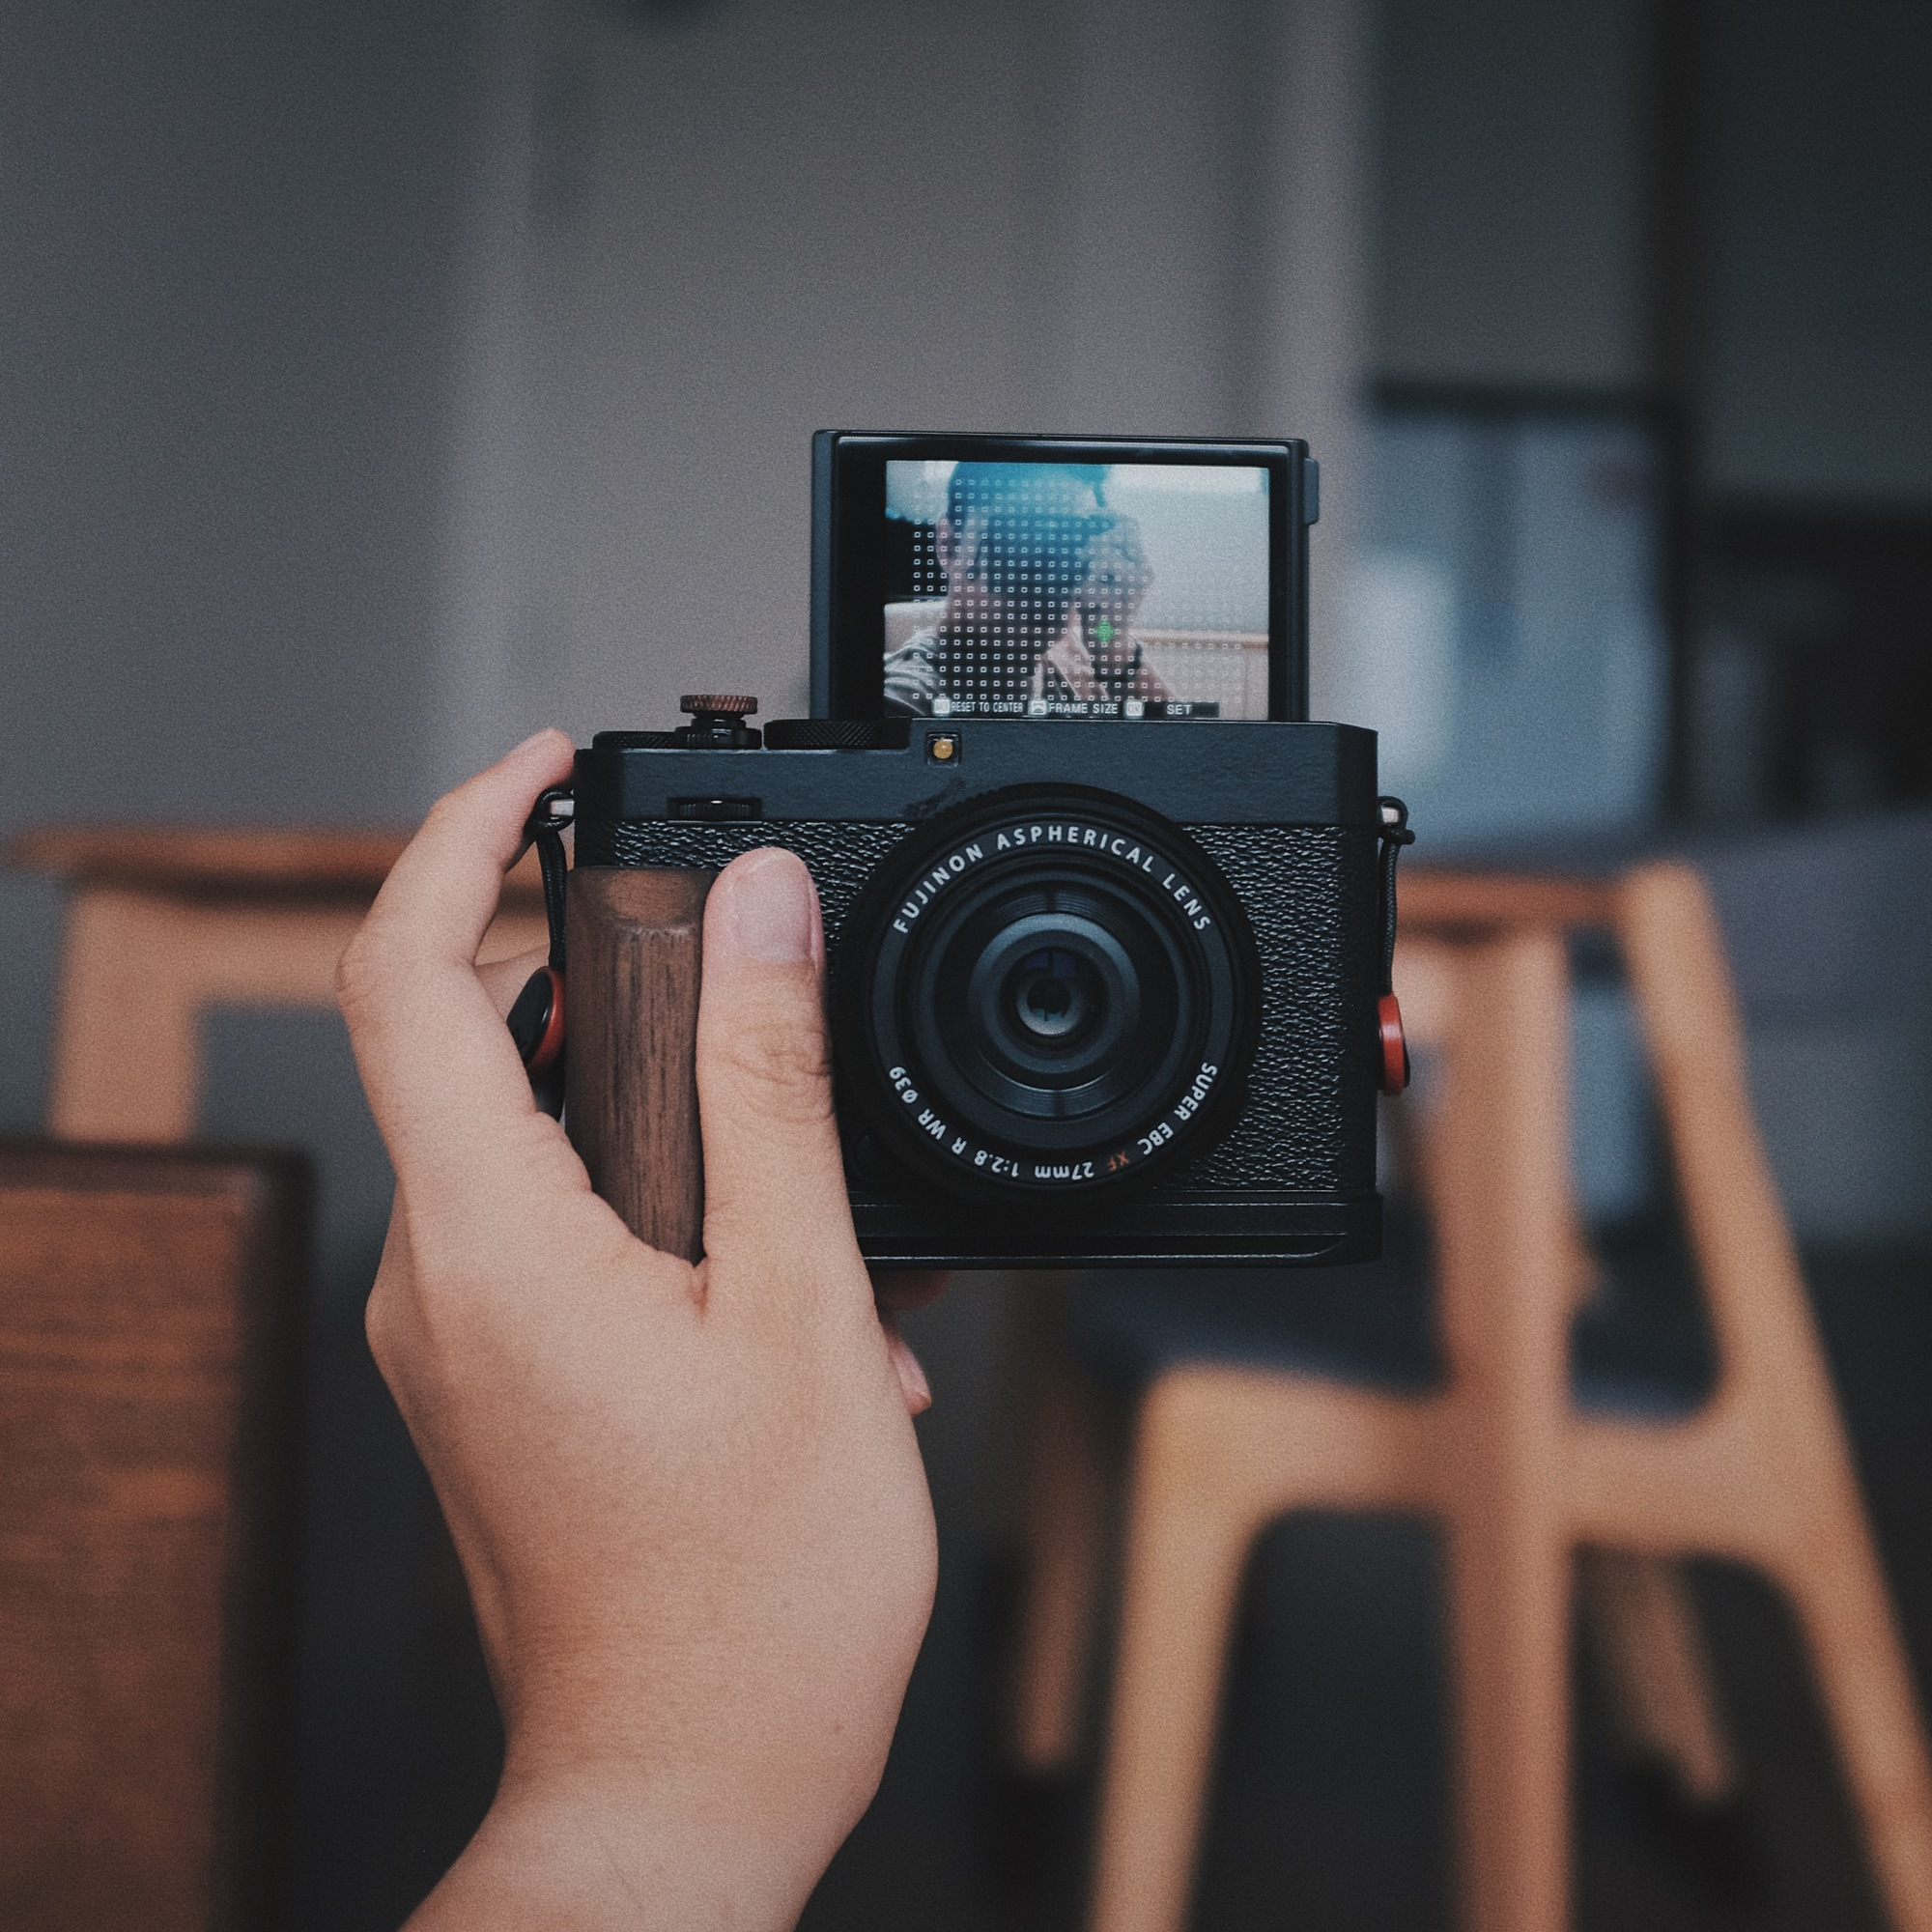
\includegraphics[width=\linewidth]{\envfinaldir/coverpic-prod.jpg}\par
            % \vskip 30pt
            \vfill

            \normalsize\rmfamily\scshape
            \copyright{} The Web Digest Project \hfill\large \envdatestr
        \end{center}
    \end{titlepage}
    % \restoregeometry
}
\newcommand{\simplehref}[1]{%
    \textcolor{blue!80!green}{\href{#1}{#1}}%
}
\renewcommand{\contentsname}{\center\Huge\sffamily\bfseries Contents\par\vskip 20pt}
\newcounter{ipartcounter}
\setcounter{ipartcounter}{0}
\newcommand{\ipart}[1]{
    % \vskip 20pt
    \clearpage
    \stepcounter{ipartcounter}
    \phantomsection
    \addcontentsline{toc}{chapter}{#1}
    % \begin{center}
    %     \Huge
    %     \sffamily\bfseries
    %     #1
    % \end{center}
    % \vskip 20pt plus 7pt
}
\newcounter{ichaptercounter}
\setcounter{ichaptercounter}{0}
\newcommand{\ichapter}[1]{
    % \vskip 20pt
    \clearpage
    \stepcounter{ichaptercounter}
    \phantomsection
    \addcontentsline{toc}{section}{\numberline{\arabic{ichaptercounter}}#1}
    \begin{center}
        \Huge
        \sffamily\bfseries
        #1
    \end{center}
    \vskip 20pt plus 7pt
}
\newcommand{\entrytitlefont}[1]{\subsection*{\raggedright\Large\sffamily\bfseries#1}}
\newcommand{\entryitemGeneric}[2]{
    % argv: title, url
    \parbox{\linewidth}{
        \entrytitlefont{#1}\par\vskip 5pt
        \footnotesize\ttfamily\mdseries
        \simplehref{#2}
    }\vskip 11pt plus 11pt minus 1pt
}
\newcommand{\entryitemGithub}[3]{
    % argv: title, url, desc
    \parbox{\linewidth}{
        \entrytitlefont{#1}\par\vskip 5pt
        \footnotesize\ttfamily\mdseries
        \simplehref{#2}\par\vskip 5pt
        \small\rmfamily\mdseries#3
    }\vskip 11pt plus 11pt minus 1pt
}
\newcommand{\entryitemAp}[3]{
    % argv: title, url, desc
    \parbox{\linewidth}{
        \entrytitlefont{#1}\par\vskip 5pt
        \footnotesize\ttfamily\mdseries
        \simplehref{#2}\par\vskip 5pt
        \small\rmfamily\mdseries#3
    }\vskip 11pt plus 11pt minus 1pt
}
\newcommand{\entryitemHackernews}[3]{
    % argv: title, hnurl, rawurl
    % \parbox{\linewidth}{
    %     \entrytitlefont{#1}\par\vskip 5pt
    %     \footnotesize\ttfamily\mdseries
    %     \simplehref{#3}\par
    %     \textcolor{black!50}{\href{#2}{#2}}
    % }\vskip 11pt plus 11pt minus 1pt
    \begin{minipage}{\linewidth}
            \entrytitlefont{#1}\par\vskip 5pt
            \footnotesize\ttfamily\mdseries
            \simplehref{#3}\par
            \textcolor{black!50}{\href{#2}{#2}}
    \end{minipage}\par\vskip 11pt plus 11pt minus 1pt
}







\begin{document}

\makeheader

\tableofcontents\clearpage




\ipart{Developers}
\ichapter{Phoronix}
\entryitemGeneric{\hskip 0pt{}Linux 6.17 Released: Intel Panther Lake Xe3 Graphics Ready, New Optimizations}{https://www.phoronix.com/news/Linux-6.17-Released}

\entryitemGeneric{\hskip 0pt{}Bcachefs Announces First-Tier Arch \& NixOS Support, Post-Experimental Release EOY}{https://www.phoronix.com/news/Bcachefs-DKMS-Announcement}

\entryitemGeneric{\hskip 0pt{}Oracle's GraalVM To Shift Focus To Non-Java Languages Like Python \& JavaScript}{https://www.phoronix.com/news/GraalVM-Non-Java-Future}

\entryitemGeneric{\hskip 0pt{}Linux 6.18 To Deliver Many Notable Features For AMD CPUs}{https://www.phoronix.com/news/Linux-6.18-AMD-CPUs}

\entryitemGeneric{\hskip 0pt{}Cryptography Performance Improvements Coming For Linux 6.18}{https://www.phoronix.com/news/Linux-6.18-Faster-Crypto}

\entryitemGeneric{\hskip 0pt{}The oneAPI Construction Kit Drops Support For Vulkan}{https://www.phoronix.com/news/oneAPI-Construction-Kit-5.0}

\entryitemGeneric{\hskip 0pt{}Fish 4.1 Released With Nearly 1,400 Commits To This Rust-Based Shell}{https://www.phoronix.com/news/Fish-4.1-Released}

\entryitemGeneric{\hskip 0pt{}Linux 6.18 Audit Code To Properly Handle Multiple Linux Security Modules}{https://www.phoronix.com/news/Linux-6.18-Audit-Subsystem}

\entryitemGeneric{\hskip 0pt{}ARM64 With Linux 6.18 To Accept Secrets From Firmware \& More}{https://www.phoronix.com/news/Linux-6.18-ARM64}


\ipart{Developers~~~~(zh-Hans)}
\ichapter{Solidot}
\entryitemGeneric{\hskip 0pt{}Firefox 将支持图像搜索}{https://www.solidot.org/story?sid=82439}

\entryitemGeneric{\hskip 0pt{}比亚迪超跑时速突破 496 km/h}{https://www.solidot.org/story?sid=82438}

\entryitemGeneric{\hskip 0pt{}Eric Schmidt 呼吁美国科技行业拥抱中国的 996 工作制}{https://www.solidot.org/story?sid=82436}

\entryitemGeneric{\hskip 0pt{}社交纽带的累积效应或有助于健康老龄化}{https://www.solidot.org/story?sid=82435}

\entryitemGeneric{\hskip 0pt{}树莓派推出 Raspberry Pi 500+}{https://www.solidot.org/story?sid=82434}

\entryitemGeneric{\hskip 0pt{}亚马逊 kindle 竭尽所能打击电子书盗版}{https://www.solidot.org/story?sid=82433}

\entryitemGeneric{\hskip 0pt{}yt-dlp 将需要安装 JS 运行时 Deno}{https://www.solidot.org/story?sid=82432}

\entryitemGeneric{\hskip 0pt{}白蚁会主动清理危害其培育鸡枞菌的有害菌}{https://www.solidot.org/story?sid=82431}

\entryitemGeneric{\hskip 0pt{}Fedora 讨论使用 AI 工具的政策}{https://www.solidot.org/story?sid=82430}

\entryitemGeneric{\hskip 0pt{}PostgreSQL 18 释出}{https://www.solidot.org/story?sid=82429}

\entryitemGeneric{\hskip 0pt{}在笔记本电脑上模拟宇宙}{https://www.solidot.org/story?sid=82428}

\entryitemGeneric{\hskip 0pt{}ROG Xbox Ally X 售价 1000 美元}{https://www.solidot.org/story?sid=82427}

\entryitemGeneric{\hskip 0pt{}OpenAI 准备建造的数据中心消耗的电力相当于纽约和圣迭戈 }{https://www.solidot.org/story?sid=82426}

\entryitemGeneric{\hskip 0pt{}微软禁止以色列国防部使用它的某些云服务}{https://www.solidot.org/story?sid=82425}

\entryitemGeneric{\hskip 0pt{}对 117 岁寿星的 DNA 研究揭示了长寿的线索}{https://www.solidot.org/story?sid=82423}

\entryitemGeneric{\hskip 0pt{}中国学者《科学》论文接受率为北美同行 1/4}{https://www.solidot.org/story?sid=82422}\ichapter{V2EX}
\entryitemGeneric{\hskip 0pt{}[游戏] Epic Games 喜+1:免费领取《Eastern Exorcist》}{https://www.v2ex.com/t/1162511}

\entryitemGeneric{\hskip 0pt{}[站长] 搞了一台 MACmini 托管到机房 拿来搞游戏服 感觉还可以}{https://www.v2ex.com/t/1162510}

\entryitemGeneric{\hskip 0pt{}[问与答] 英语遇到瓶颈求建议}{https://www.v2ex.com/t/1162509}

\entryitemGeneric{\hskip 0pt{}[iPhone] iPhone Pro 上面的 USB3 用处大吗?}{https://www.v2ex.com/t/1162508}

\entryitemGeneric{\hskip 0pt{}[分享创造] Hello 👋,来带货一下最近写的 web3 shell client,已开源~}{https://www.v2ex.com/t/1162507}

\entryitemGeneric{\hskip 0pt{}[分享创造] 远离 ratio 焦虑,我写了一个 PT 免费下载小工具}{https://www.v2ex.com/t/1162506}

\entryitemGeneric{\hskip 0pt{}[求职] 上海 - 6 年数据研发 - 求职}{https://www.v2ex.com/t/1162504}

\entryitemGeneric{\hskip 0pt{}[分享创造] 做了一个将自拍转成 恐怖片风格的工具}{https://www.v2ex.com/t/1162503}

\entryitemGeneric{\hskip 0pt{}[分享创造] 用 Python 实现了一个局域网内手机远程控制电脑的功能}{https://www.v2ex.com/t/1162502}

\entryitemGeneric{\hskip 0pt{}[宽带症候群] 国内是不是已经完全禁止了 openvpn 的链接使用?}{https://www.v2ex.com/t/1162501}

\entryitemGeneric{\hskip 0pt{}[Apple] iOS 26 之后 14pro 的 wifi 信号变得稳定了}{https://www.v2ex.com/t/1162500}

\entryitemGeneric{\hskip 0pt{}[Local LLM] 本地部署了大模型如何有效利用?}{https://www.v2ex.com/t/1162498}

\entryitemGeneric{\hskip 0pt{}[分享创造] Gemini 创意玩法——彼得林奇投资 Agent}{https://www.v2ex.com/t/1162497}

\entryitemGeneric{\hskip 0pt{}[问与答] LLM 调用 MCP 的机制到底是什么?为什么有些 MCP 安装了却不调用?}{https://www.v2ex.com/t/1162496}

\entryitemGeneric{\hskip 0pt{}[Apple] iCloud 相册里面的视频导出为 MOV 和 xmp 文件后,再导出,是不是就丢失了信息?(因为 xmp 文件无法导入)}{https://www.v2ex.com/t/1162495}

\entryitemGeneric{\hskip 0pt{}[Android] 有用小米 17 系列的吗?想问问你们的「账号与同步」中的「自动同步数据」开关会不会莫名其妙自己关闭啊?}{https://www.v2ex.com/t/1162494}

\entryitemGeneric{\hskip 0pt{}[Apple] 官网刚办完分期,还能退吗}{https://www.v2ex.com/t/1162492}

\entryitemGeneric{\hskip 0pt{}[分享发现] [网站自荐] BLOODMONEY!:最黑暗的点击游戏,\$25,000 绝望目标与三线结局}{https://www.v2ex.com/t/1162491}

\entryitemGeneric{\hskip 0pt{}[程序员] 从产品角度评价 v2ex}{https://www.v2ex.com/t/1162490}

\entryitemGeneric{\hskip 0pt{}[问与答] PgSQL 和 Sqlserver 哪个好?哪个资源占用小?哪个性能好速度快?}{https://www.v2ex.com/t/1162489}

\entryitemGeneric{\hskip 0pt{}[分享发现] [征友链] 一起互挂链接,交个朋友 🚀}{https://www.v2ex.com/t/1162487}

\entryitemGeneric{\hskip 0pt{}[问与答] 无忧行企业版 callkit 接电话没声音咋办?}{https://www.v2ex.com/t/1162486}

\entryitemGeneric{\hskip 0pt{}[Android] Google Pixel 更新后或将不再支持中国运营商}{https://www.v2ex.com/t/1162485}

\entryitemGeneric{\hskip 0pt{}[分享发现] 分享两个四川电信维权案例}{https://www.v2ex.com/t/1162484}

\entryitemGeneric{\hskip 0pt{}[随想] 观《湾区升明月》晚会有感}{https://www.v2ex.com/t/1162483}

\entryitemGeneric{\hskip 0pt{}[问与答] 禁用了输入法 App 的联网权限,为什么依然每天都有数据产生?}{https://www.v2ex.com/t/1162482}

\entryitemGeneric{\hskip 0pt{}[问与答] 中秋送礼和自己食用,求推荐一些无糖月饼.只要无糖即可, 其他口味不限.}{https://www.v2ex.com/t/1162481}

\entryitemGeneric{\hskip 0pt{}[问与答] 大佬们,电脑键盘漏电,人麻了~}{https://www.v2ex.com/t/1162480}

\entryitemGeneric{\hskip 0pt{}[问与答] AWS SES 邮件这么难通过吗?}{https://www.v2ex.com/t/1162479}

\entryitemGeneric{\hskip 0pt{}[问与答] 想问下大家怎么使用 Apple watch 提高效率呢?}{https://www.v2ex.com/t/1162476}

\entryitemGeneric{\hskip 0pt{}[分享创造] SwiftyMenu 26 一键启动 Claude Code, Codex CLI, Copilot Agent...}{https://www.v2ex.com/t/1162475}

\entryitemGeneric{\hskip 0pt{}[Claude] Claude Pro 账户如何使用 Claude Code?}{https://www.v2ex.com/t/1162474}

\entryitemGeneric{\hskip 0pt{}[问与答] 阿里云的这个发票是认真的吗?注意避坑了}{https://www.v2ex.com/t/1162472}

\entryitemGeneric{\hskip 0pt{}[分享创造] 开发了个插件,用来快速在 visual studio 和 Cursor 之间切换}{https://www.v2ex.com/t/1162471}

\entryitemGeneric{\hskip 0pt{}[分享创造] 想做一个《个人记忆体》的 ai ,有多少人有兴趣}{https://www.v2ex.com/t/1162470}

\entryitemGeneric{\hskip 0pt{}[职场话题] 外包就外包,外协岗是什么?}{https://www.v2ex.com/t/1162469}

\entryitemGeneric{\hskip 0pt{}[职场话题] 组里来了三个华为的之后,越来越卷了,工时高的快卷到 250 小时(减去中午下午休息两小时后)了。}{https://www.v2ex.com/t/1162466}

\entryitemGeneric{\hskip 0pt{}[iPhone] 安卓转苹果,问几个问题}{https://www.v2ex.com/t/1162464}

\entryitemGeneric{\hskip 0pt{}[Claude] 1 个月前购买的 claude code 被封号了}{https://www.v2ex.com/t/1162463}

\entryitemGeneric{\hskip 0pt{}[奇思妙想] 做一个业务层的 ratelimit saas 服务是否可行}{https://www.v2ex.com/t/1162462}

\entryitemGeneric{\hskip 0pt{}[职场话题] 一个超离谱的事,一个超离谱的员工}{https://www.v2ex.com/t/1162461}

\entryitemGeneric{\hskip 0pt{}[成都] 国庆去重庆玩怎么样?}{https://www.v2ex.com/t/1162460}

\entryitemGeneric{\hskip 0pt{}[随想] 未来百年的一个人类效率提升点会不会发生在数字到生物}{https://www.v2ex.com/t/1162458}

\entryitemGeneric{\hskip 0pt{}[问与答] 有什么办法通过软件关闭台式机的所有灯光吗}{https://www.v2ex.com/t/1162457}

\entryitemGeneric{\hskip 0pt{}[酷工作] 上海游戏厂 sre 工程师 HC! T0 员工福利待遇~}{https://www.v2ex.com/t/1162456}

\entryitemGeneric{\hskip 0pt{}[问与答] 我想知道为什么我现在发一个帖子要 105 铜币,以前发帖子只要 20 铜币}{https://www.v2ex.com/t/1162455}

\entryitemGeneric{\hskip 0pt{}[生活] 9 月已经到月底了,关于幼儿园大班免费你们的城市都是什么政策。}{https://www.v2ex.com/t/1162453}

\entryitemGeneric{\hskip 0pt{}[问与答] 为什么马路三大妈总喜欢占用快车道,又慢又占道,这些车主是什么心态?}{https://www.v2ex.com/t/1162452}

\entryitemGeneric{\hskip 0pt{}[iPhone] 已经收到 iPhone 17 系列的朋友可以说说使用体验怎么样吗?}{https://www.v2ex.com/t/1162451}

\entryitemGeneric{\hskip 0pt{}[问与答] 帖子列表中间的深入探索是干啥的呀?}{https://www.v2ex.com/t/1162450}


\ipart{Generic News}







\clearpage
\leavevmode\vfill
\footnotesize

Copyright \copyright{} 2023-2025 Neruthes and other contributors.

This document is published with CC BY-NC-ND 4.0 license.

The entries listed in this newsletter may be copyrighted by their respective creators.

This newsletter is generated by the Web Digest project.

The newsletters are also delivered via Telegram channel \CJKunderline{\href{https://t.me/webdigestchannel}{https://t.me/webdigestchannel}}.\\
RSS feed is available at \CJKunderline{\href{https://webdigest.pages.dev/rss.xml}{https://webdigest.pages.dev/rss.xml}}.

This newsletter is available in PDF at
\CJKunderline{\href{https://webdigest.pages.dev/}{https://webdigest.pages.dev/}}.

The source code being used to generate this newsletter is available at\\
\CJKunderline{\href{https://github.com/neruthes/webdigest}{https://github.com/neruthes/webdigest}}.

This newsletter is also available in
\CJKunderline{\href{http://webdigest.pages.dev/readhtml/\envyear/WebDigest-20250929.html}{HTML}} and
\CJKunderline{\href{https://github.com/neruthes/webdigest/blob/master/markdown/\envyear/WebDigest-20250929.md}{Markdown}}.


\coverpic{https://unsplash.com/photos/modern-apartment-building-facade-with-balconies-and-balconies-9NNAR40GXVM}{Sebastian Schuster}


\end{document}
